\documentclass[8pt]{extarticle}
\usepackage{makeidx}
\usepackage{graphicx}
\usepackage{amsmath}
\usepackage{amssymb}
\usepackage{caption}
\usepackage{subcaption}
\usepackage{latexsym}
\renewcommand\refname{Referenze}
\usepackage[utf8x]{inputenc}
\usepackage{titlesec}
\usepackage{bm}
\usepackage{mathtools}
\usepackage[document]{ragged2e}
\titleformat{\section}{\huge\normalfont\bf}{\thesection.\hspace{5pt}}{5pt}{\vspace{1cm}}
\titleformat*{\subsection}{\Large\bfseries}
\usepackage[inner=3cm,outer=3cm]{geometry}

\makeindex

\begin{document}
\justify
\printindex
\Large{A.a. 2013-2014}
\vspace{10cm}
\begin{center}
\Huge\textbf{Tracciamento dei Raggi Cosmici}
\end{center}

\vspace{2cm}
\begin{flushleft}
\textit{Gruppo \textsc{1}} \\
\medskip
Federico \textsc{Massa} \\ 
Marco \textsc{Montella}
\end{flushleft}



\newpage

\begin{abstract}
\justify
 

\end{abstract}
\bigskip

\section{Introduzione} \label{sec:intro}
L'esperimento consiste nell'analisi dei dati provenienti da un telescopio per raggi cosmici facente parte del progetto \textit{Extreme Energy Events} (EEE). L'apparato è composto da un sistema di tre camere MRPC, grazie alle quali è possibile registrare il passaggio di una particella e le coordinate di arrivo su ognuna delle tre camere. Utilizzando questo sistema sono state effettuate varie misure: \\

\begin{enumerate}
\item Misura dell'efficienza dei piani di scintillatore in funzione della tensione di alimentazione.
\item Misura del flusso di raggi cosmici.
\item Misura della distribuzione angolare dei raggi cosmici.
\item Studio della correlazione tra condizioni ambientali e il flusso dei raggi cosmici.
\end{enumerate}

Precedenti studi\cite{cos2} hanno misurato una distribuzione angolare dei raggi cosmici compatibile con la legge: \\

\begin{equation}
\frac{dN}{d\Omega} \propto cos^2 \theta
\nonumber
\end{equation}

dove $\theta$ è l'angolo formato tra la retta identificante la traiettoria della particella e la normale alla superficie terrestre. \\

Una parte dell'esperimento consiste pertanto nella simulazione, con metodi Montecarlo, della distribuzione angolare dei raggi cosmici che risultano in un effettivo segnale nell'apparato. La simulazione ha anche tenuto conto di alcuni difetti riscontrati nell'apparato (\textit{strip} delle camere non funzionanti) e della discretizzazione della coordinata trasversale alla direzione delle strip. \\

\section{Apparato Sperimentale}
\subsection{Rivelatore a camere MRPC}
Il sistema consiste di tre \textit{Multi-gap Resistive Plate Chamber} (MRPC). La struttura di una di queste camere è mostrata in fig. \ref{fig:mrpc}. \\

\begin{figure}
\begin{center}
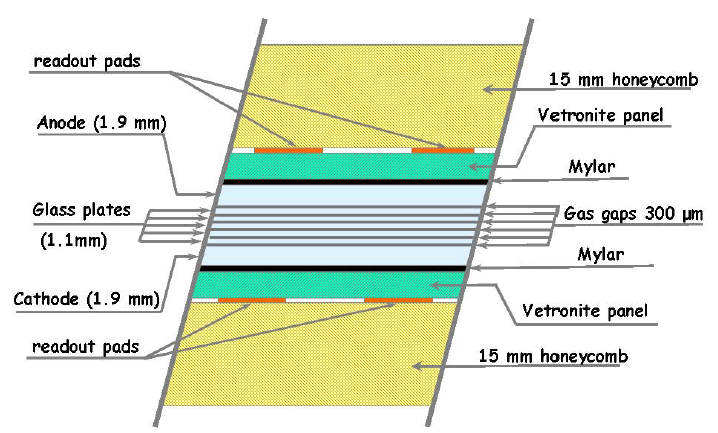
\includegraphics[scale=0.3]{mrpc}
\caption{Sezione trasversale di una camera MRPC.}
\label{fig:mrpc}
\end{center}
\end{figure}

Una particolare miscela di gas è contenuta all'interno di sei strati di vetro spessi $1.1 \ mm$, ognuno distante $300 \mu \ m$. Gli strati più esterni sono tenuti ad una certa differenza di potenziale, mentre gli strati interni si caricano per effetto dell'induzione elettrostatica. \\
Quando una particella carica attraversa il sistema il gas viene ionizzato e la differenza di potenziale accelera gli elettroni i quali possono acquistare un'energia sufficiente a 
provocare una valanga di elettroni secondari. L'insieme di questi elettroni induce un segnale su una o più \textit{strips} (\textit{readout pads} nella figura). Il sistema è composto da $24$ strip, ognuna larga $3.2 \ cm$ e l'area attiva misura $82 \ x \ 158 \ cm^2$. La distanza tra la camera in alto e quella media è $53.2 \ cm$, mentre la distanza tra quella media e quella in basso è $52.8 \ cm$.  Il resto degli elementi che compongono la camera sono strutturali o isolanti. \\

\subsection{Sistema di acquisizione}
Il segnale in uscita dalle strip viene digitalizzato da un'opportuna unità di Front-End e viene generato un segnale di trigger che potrà essere configurato via software per la selezione degli eventi.\\

Le coordinate $(x,y)$ della particella sono ricostruite su un asse a partire dalla coordinata della strip che ha generato un segnale, sull'altro dall'analisi della differenza dei tempi di arrivo del segnale ai due estremi della strip. Le incertezze sono state stimate dai dati sperimentali, come descritto in sez. \ref{subsec:coord_err}. \\

La coordinata y (quella relativa alla direzione parallela alle strip) è calcolabile, una volta nota la velocità di propagazione del segnale $v_s$, dalla relazione: \\
\[y = \frac{v_s}{2} (t_s - t_d) \] \\

dove $t_s$ e $t_d$ indicano i tempi di arrivo sui due estremi della strip. \\
Un TDC (Time-to-Digital Converter) permette l'acquisizione in formato digitale di queste grandezze, da cui viene calcolato il valore della coordinata. \\

Una serie di sensori di pressione, umidità e temperatura possono infine essere utilizzati per avere informazioni sulle condizioni ambientali al momento della presa dati.

\subsection{Interfaccia software}
Il processo di acquisizione è configurabile via software. Grazie ad un'interfaccia dedicata è possibile impostare parametri di acquisizione quali: \\
\begin{itemize}
\item Tensioni di alimentazione delle camere.
\item Segnale di trigger.
\item Numero di eventi da acquisire.
\end{itemize}

Le istruzioni possono anche essere riassunte in macro che permettono di automatizzare il processo.\\

In uscita vengono restituiti i seguenti files: \\
\begin{enumerate}
\item \textbf{.dat}: contiene i dati provenienti dal sistema di acquisizione in formato binario, non processati.
\item \textbf{.sta}: contiene i dati, sempre in formato binario, provenienti dai sensori e dalle letture di tensione.
\item \textbf{.arc}: file di testo contente le informazioni sulla geometria del sistema, sul nome e ID del run.
\item \textbf{.txt}: file di testo contenente le coordinate dei punti evento per evento e i valori delle letture dei sensori.
\item \textbf{.sto}: file contenente una prima analisi dei risultati del run. Contiene informazioni quali le distribuzioni di occupancy nelle tre camere, la molteplicità di hit e i risultati di altre analisi condotti sugli eventi che presentano un solo hit per ogni camera, i quali non sono però stati utilizzati.
\end{enumerate}

Di questi, il fondamentale è quello \textbf{.txt}, ed è stato l'unico utilizzato nel corso dell'esperimento.

\subsection{Scintillatori}
Due scintillatori sono stati posizionati sopra e sotto il sistema di tracciamento. La loro misura è $44 \ x \ 125.5 cm^2$. Lo scintillatore posto sopra il sistema dista $37.5 \ cm$ dalla camera alta, mentre lo scintillatore posto sotto il sistema dista $16 \ cm$ dalla camera bassa. Gli scintillatori sono opportunamente alimentati, il loro segnale è digitalizzato ed è possibile utilizzare uno di questi o la loro coincidenza come segnale di trigger per il sistema di acquisizione. Il sistema così configurato è stato utilizzato per delle verifiche sulle misure di efficienza delle camere MRPC.

\section{Operazioni preliminari}
È stata effettuata un’analisi preliminare dei dati raccolti allo scopo di cercare eventuali anomalie macroscopiche nel funzionamento delle camere, come ad esempio eventuali strip mancanti o rumorose. Allo stesso tempo si è condotta un'analisi dell'efficienza delle tre camere in funzione della tensione di alimentazione ai capi delle strip (è questa l'alimentazione IMPORTANTE??). INTRO ALL'INCERTEZZA

\subsection{Correzioni geometriche}
Le coordinate dei punti nel file in uscita non corrispondo a quelle reali della camera. Per correggere questo effetto è stato considerato il file corrispondente a un run ad alta statistica e, per ogni camera, è stata guardata la distribuzione di occupancy sul piano XY. Da questa distribuzione sono state estratte le posizioni delle strip (per quanto riguarda la coordinata x) e i valori estremi che assume la coordinata y per ogni strip. In realtà nella distribuzione precedente alla correzione, mostrata in fig. \ref{fig:disxy1_prima}, si vede che le coordinate y non hanno un limite perfettamente definito. \'E possibile, infatti, che tra i valori restituiti ve ne siano alcuni che derivano da eventi di rumore nel TDC. I valori degli estremi sono stati ricavati cercando i punti in cui l'istogramma assume valori nulli per più di un bin consecutivo. Una volta applicate le traslazioni per ogni camera e per ogni strip, i valori sono stati riscalati alle dimensioni reali delle camere. Il risultato è mostrato in fig. \ref{fig:disxy1_dopo}.

\begin{figure}
\centering
\begin{subfigure}{.5\textwidth}
  \centering
  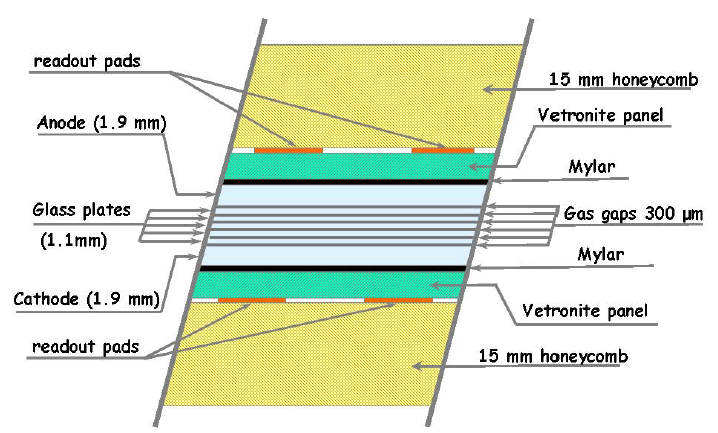
\includegraphics[width=.6\linewidth]{mrpc}
  \caption{Analisi del file originale.}
  \label{fig:disxy1_prima}
\end{subfigure}%
\begin{subfigure}{.5\textwidth}
  \centering
  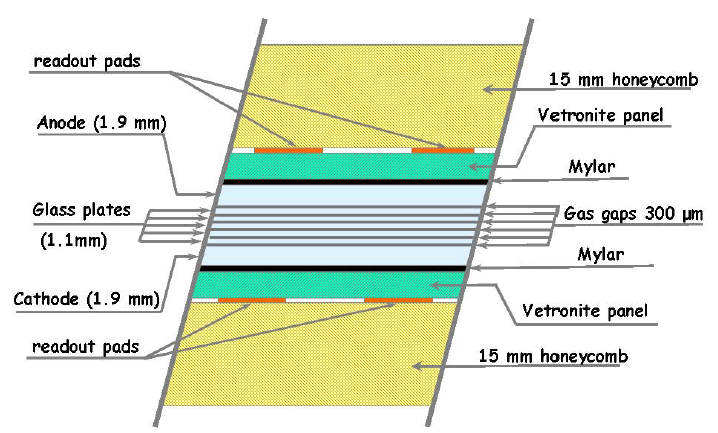
\includegraphics[width=.6\linewidth]{mrpc}
  \caption{Analisi del file corretto.}
  \label{fig:disxy1_dopo}
\end{subfigure}
\caption{Occupancy della camera 1 prima e dopo la correzione.}
\label{fig:disxy1}
\end{figure}

\subsection{Stima dell'incertezza sulle coordinate} \label{subsec:coord_err}
\'E stato utilizzato il metodo suggerito in \cite{articolo_EEE}. Analizzando le sole tracce con un hit per camera, è stata misurata la distribuzione delle quantità: \\

\[ \Delta_x = \frac{x_{F,1} + x_{F,3}}{2} - x_2 \]
\[ \Delta_y = \frac{y_{F,1} + y_{F,3}}{2} - y_2 \]

dove con il pedice $F$ si indica la coordinata relativa ad una retta ottenuta con un fit, mentre il pedice numerico indica il numero della camera corrispondente sulla quale tale coordinata è stata misurata. Questa quantità, quando misurata su un evento legittimo, si distribuisce attorno a zero a causa della risoluzione sperimentale: \\

\[ \sigma_\Delta = \sqrt{\frac{3}{2}} \ \sigma_x  \]

da cui si può ricavare $\sigma_x$.

I risultati sono mostrati, per le due coordinate, in fig. \ref{fig:errx}, \ref{fig:erry}.

\begin{figure}
\centering
\begin{subfigure}{.5\textwidth}
  \centering
  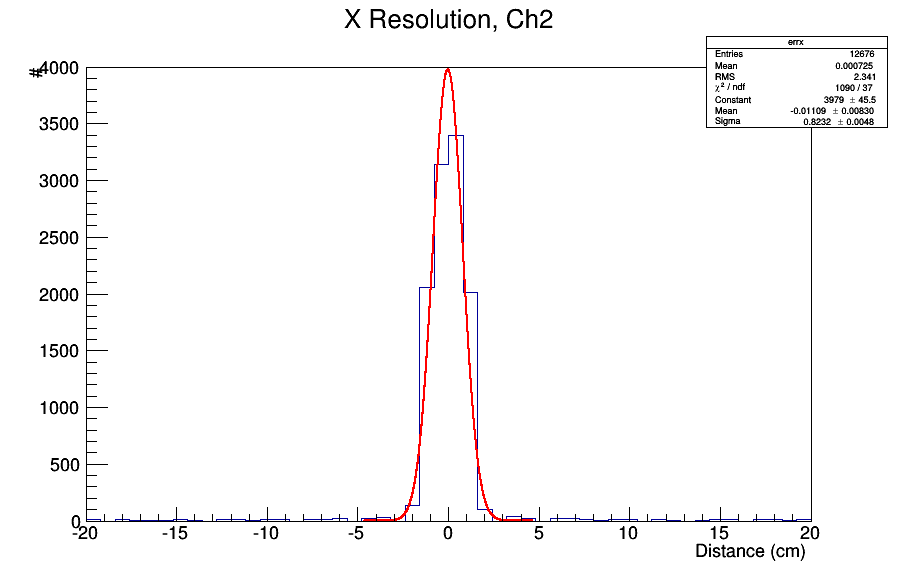
\includegraphics[width=1\linewidth]{errx}
  \caption{Distribuzione di $\Delta_x$.}
  \label{fig:errx}
\end{subfigure}%
\begin{subfigure}{.5\textwidth}
  \centering
  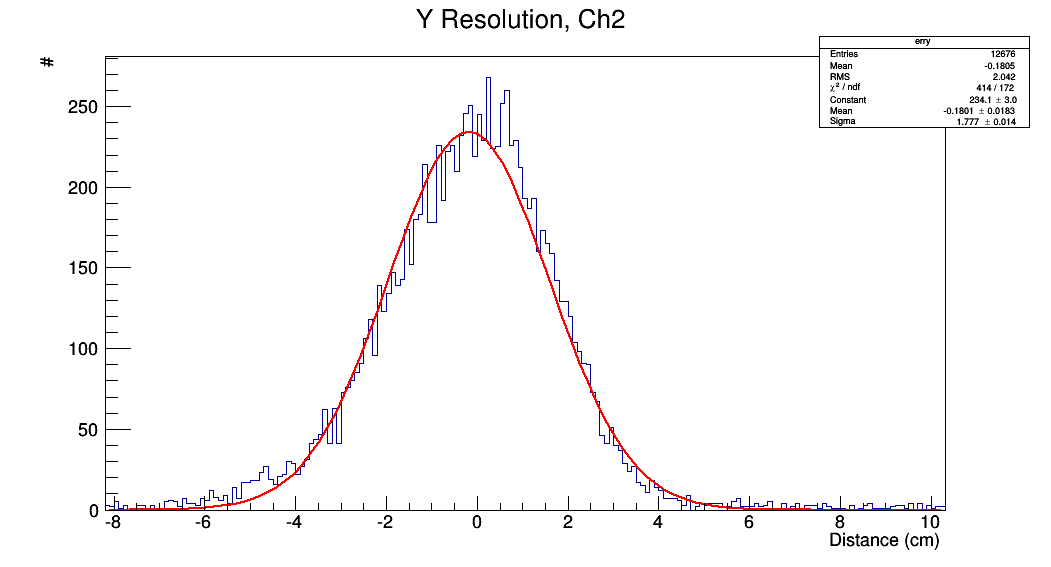
\includegraphics[width=1\linewidth]{erry}
  \caption{Distribuzione di $\Delta_y$ e relativo fit gaussiano.}
  \label{fig:erry}
\end{subfigure}
\caption{Distribuzioni per il calcolo dell'incertezza sulle coordinate.}
\label{fig:err_coordinate}
\end{figure}

Per la coordinata z, che dipende dallo spessore della regione attiva, si è considerata una distribuzione uniforme. Le incertezze risultanti sono riassunte di seguito:\\

\[ \sigma_x = 0.7 \ cm \]
\[ \sigma_y = 1.6 \ cm \]
\[ \sigma_z = 0.2 \ cm \]

\subsection{Misure di Occupancy}
Nel contesto dell'analisi del  corretto funzionamento delle camere si sono ricostruite all'interno di un run le distribuzioni di occupancy per ciascuna camera nella variabile direzionale discreta X (strip interessata/e) e continua Y (conteggi del TDC), al fine di identificare eventuali zone morte del rivelatore o regioni con una sospetta accumulazione di hits.\\
(GRAFICI, SULLE SINGOLE CAMERE ETC, FARLI PICCOLI, SONO TANTI)
(SCRIVERE QUALI SONO LE STRIP MANCANTI)
(PRENDERE UN AND ALL PER QUESTA ANALISI, È PIÙ FACILE GIUSTIFICARE LA FORMA A CAMPANA O UNIFORME)

In secondo luogo si è osservata la molteplicità di hit per evento in ciascuna camera, rilevando un trend rapidamente decrescente. [INSERIRE LE FRAZIONI DI EVENTI CON 1 HIT PER CAMERA, 2 HIT E COSÌ VIA]. 
[DISCERNERE HIT MULTIPLI DI RUMORE DA QUALCOSA DI SEGNALE, GLI ALTRI PIANI QUANTO CONTANO QUANDO UNO CONTA MOLTO?]

\subsection{Distribuzione delle distanze tra due hit in ciascuna camera} \label{subsec:dis_corr}
Si sono poi valutate, all'interno di un run, la distanza geometrica tra gli hit di ciascun evento  sia sulle due dimensioni che sulle singole direttrici del piano. Ci si attende una distribuzione identificabile come somma di due componenti distinte, una ragionevolmente piatta dovuta agli hit non correlati e una piccata su un valore $d_0$ relativa agli eventi per cui gli hit multipli derivano da una comune causa fisica (che sia essa di segnale o di rumore). 
Nel caso descritto sarebbe inoltre possibile definire una distanza di correlazione $d_c$ che rappresenta la distanza a cui si trovano all'incirca il 90\% delle coppie di hits appartenenti alla distribuzione di hits fisicamente correlati. Il risultato, mostrato in fig. \ref{fig:dis_correlazione}, porta alla misura: \\
\[ d_c = 14 cm \]

\begin{figure}
\begin{center}
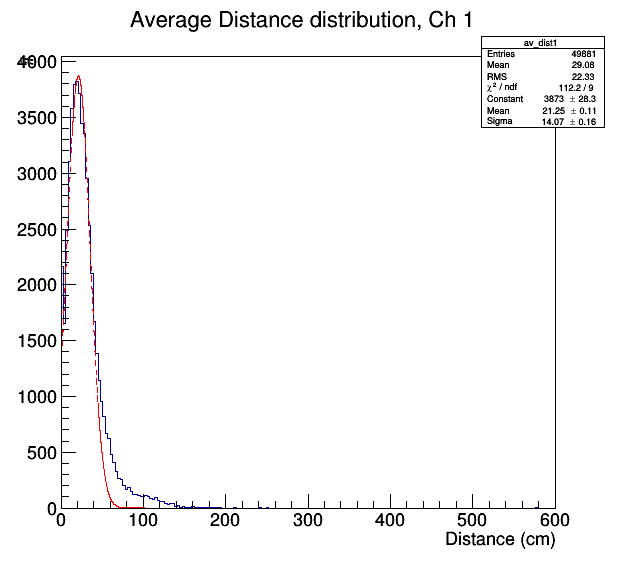
\includegraphics[scale=0.3]{dis_correlazione}
\caption{Distribuzione delle distanze tra tutte le coppie di hit all'interno di un run nella camera 1 (esempio).}
\label{fig:dis_correlazione}
\end{center}
\end{figure}


\subsection{Misure di efficienza}
Le misure di efficienza delle camere possono effettuate secondo modalità molteplici. L'efficienza del piano centrale può essere calcolata in modo immediato esaminando dati acquisiti con la modalità di trigger \textit{TOP-BOTTOM}, ovvero richiedendo la presenza di un hit nelle camere esterne per la registrazione di un evento, e valutando il numero di eventi per i quali viene anche ravvisato uno o più hit nella camera centrale. \\
Lo stesso metodo non può però essere applicato nel calcolo delle efficienze dei piani estremi, in quanto una particella non passante il piano oggetto dell'analisi può comunque attraversare i due rimanenti e far scattare il trigger, falsando il risultato.
\subsubsection{Efficienza con ricostruzione tracce}
Questo problema viene aggirato utilizzando una variante dell'algoritmo di ricostruzione delle tracce che sarà descritto nel dettaglio in sezione (\ref{subsub:algoritmo}). L'algoritmo ricostruisce la traccia a partire dalle coppie di hit nei piani spettatori e determina se esiste un hit nella camera in analisi che conduca ad un fit a tre punti accettabile. Qualora il prolungamento della traccia virtuale determinata dagli hit sui piani spettatori cada al di fuori della zona attiva del piano in analisi l'evento viene scartato senza incidere sul calcolo dell'efficienza.
[GRAFICI]
[GRAFICI IN FUNZIONE DELLA TENSIONE]

\subsubsection{Uso degli scintillatori}
\'E possibile effetturare una seconda stima delle efficienze sfruttando un sistema alternativo di trigger. \\
Per realizzare tale trigger alternativo si fa uso di due piani scintillatori esterni all'apparato di dimensione 44x120 cm precedentemente calibrati e messi in tempo dal personale responsabile e posizionati uno al di sopra del piano superiore e uno al di sotto del piano più vicino al suolo. Il segnale di trigger per l'acquisizione nelle tre camere  MRPC viene dato dalla coincidenza dei segnali di output dei due scintillatori. \\
Il calcolo effettivo dell'efficienza utilizzando i dati acquisiti con il metodo appena descritto può essere condotta facendo o meno uso della ricostruzione delle tracce.
Qualora i valori di efficienza calcolati con il trigger esterno non fossero compatibili con le misure delle medesime quantità effettuate in precedenza si avrebbe un indizio della possibile presenza di un problema nel sistema di trigger dell'apparato.\\
(VALORI EFFICIENZE, GRAFICO VARIAZIONE CON LA TENSIONE, GRAFICO PARAGONE TRIGGER ESTERNO O INTERNO)

\section{Simulazione}

\subsection{Calcolo dell'accettanza}
In primo luogo è stato sviluppato un programma in C++ interfacciato in ROOT per calcolare l’accettanza dell’apparato note le caratteristiche geometriche e di efficienza delle aree sensibili dei tre piani di rivelazione.//
In questo modo si è inoltre potuto valutare la distribuzione teorica dei raggi cosmici accettati nell’angolo polare $\theta$ e nell’angolo azimutale $\phi$. \\
Le misure di efficienza dei singoli piani effettuati in precedenza sono state implementate nel calcolo dell'accettanza, permettendo così di ottenere un coefficiente moltiplicativo realistico grazie al quale stimare, a partire dai dati di flusso, la frazione misurata del rate di raggi cosmici.

Il calcolo dell'accettanza è stato effettuando generando un numero fissato di tracce secondo la distribuzione angolare teorica della componente hard dei raggi cosmici, e determinando in seguito la frazione di tali tracce in grado di produrre un segnale nell'apparato.\\
La procedura è schematizzata nei seguenti steps:
\begin{itemize}
\item Generazione della coppia $(\theta, \phi)$ secondo le rispettive distribuzioni come note dalla teoria.
\item Generazione del punto di impatto sulla camera centrale secondo una distribuzione uniforme.
\item Determinazione delle intersezioni della traccia generata con i piani su cui giacciono le restanti due camere.
\item Controllo di appartenenza di tali punti all'area attiva del rivelatore.
\item Controllo di efficienza per le tre camere.
\end{itemize}


%La forma di quest’ultima distribuzione risulta fortemente dipendente dalle caratteristiche geometriche del singolo piano, e la di essi forma rettangolare causa  la presenza di un massimo dell’accettanza differenziale in phi lungo la direzione del lato maggiore.
%La distribuzione in phi è inoltre più sensibile ad un eventuale cattivo allineamento dei tre piani, secondo modalità tuttora da indagare appieno. 

\subsection{Effetto della discretizzazione della coordinata X}
Si è in seguito deciso di modificare il software di simulazione in modo da tenere conto della quantizzazione dei valori della coordinata X dovuta alla presenza di un numero limitato di strip.\\
Per fare ciò la dimensione X di ciascun piano è stata idealmente divisa in 24 sezioni adiacenti centrate ciascuna sull'asse della relativa strip, e comprendente agli estremi metà della regione tra la strip e le sue adiacenti. I punti generati sono stati a questo punto corretti re-impostando la coordinata X di ciascuno con la coordinata X centrale della strip di competenza. \\
L'effetto della discretizzazione della coordinata trasversale alle strip sulle distribuzioni dei $\theta$ e dei $\phi$ accettati è mostrato nelle figure sottostanti.
[figura theta]
[figura correlazione]
Si nota come le due distribuzioni risultano compatibili su quasi tutto lo spettro in $\theta$, con la quantità $\theta_{disc}-\theta$ che si presenta decrescente al crescere di $\theta$, ma limitata a $\pm 1°$ per $\theta>4°$. Si osserva invece che gli eventi con $\theta < 4°$ subiscono una correzione più importante, fino a circa 5°. Tale riscontro è plausibile in quanto un uguale $\Delta x$, rappresentato dall'errore massimo sulla posizione X introdotto dalla discretizzazione, influisce tanto di più sulla variazione dei parametri di pendenza del fit lineare quanto più la retta tende alla verticalità.\\

Nella figura [figura phi] sono invece mostrate le distribuzioni prima e dopo la discretizzazione delle X per l'angolo azimutale $\phi$. L'effetto, ben più macroscopico rispetto all'angolo polare, si traduce in un aumento del numero di eventi con $\phi$ riconosciuto pari a 90° o a 270° e in una diminuzione sensibile degli eventi con angoli distanti fino a 15° dai due valori citati sopra.\\
Questo effetto è stato studiato separatamente correlando, per gli eventi per cui vale $|\phi-(90,270)|\leq 15°$, la differenza $\phi_{disc}-\phi$ con l'angolo $\theta$, come mostrato nella [FIGURAA].\\
L'errore sulla determinazione dell'angolo $\phi$ è anche in questo caso massimo, con $\Delta phi_{max}\sim \pm 90°$, per le tracce con $\theta \sim 0°$. \\
L'angolo $\phi$ è infatti calcolato a partire dalla traccia proiettiva sul piano XY, e i tre punti di tale traccia proiettiva risulteranno tanto più ravvicinati sul piano quanto più $\theta$ tende a zero. In tale condizione è facile che le ascisse dei tre punti della traccia cadano nella zona di influenza della medesima strip, facendo si che l'algoritmo di estrazione dell'angolo $\phi$, basato sul fit della traccia proiettiva XY, restituisca 90° o 270° (corrispondenti a proiezioni verticali sul piano XY) a prescindere dall'effettivo valore di $\phi$.
\subsection{Effetto delle strip mancanti}
Le precedenti analisi di occupancy hanno mostrato come un certo numero di strip in ciascuna delle tre camere non risultino funzionanti. Il calcolo dell'accettanza deve dunque tenere conto di tale deficit per poter produrre un valore realistico. Si ottiene:\[A_{corr}=0.1783\].
L'asimmetria nella disposizione spaziale delle strip mancanti è causa di un effetto sistematico sulla distribuzione degli angoli accettati, evidente in particolare nel caso dell'angolo $\phi$. Si ha infatti per l'angolo azimutale, una diminuzione sistematica della frazione di eventi accettati con angolo compreso tra 90° e 270°. Le distribuzioni dell'angolo $\theta$ sono invece compatibili.

\section{Metodo di misura}

\subsection{Determinazione della distribuzione angolare dei RC}

\subsubsection{Ricostruzione delle tracce}



\subsubsection{Ricostruzione delle tracce} \label{subsub:algoritmo}
L’acquisizione delle misure è per il momento effettuata in modalità AND ALL, ovvero impostando il trigger sulla coincidenza dei segnali provenienti dalle tre camere. Nonostante ciò nei file ad alta statistica sono comunque presenti un certo numero di eventi senza almeno un hit per camera, i quali vengono ignorati nel seguito dell’analisi.\\
Gli eventi che rispettano la condizione di trigger vengono analizzati con un software in linguaggio C++ interfacciato ROOT finalizzato alla ricostruzione della traccia eventuale e all’estrapolazione dei parametri angolari della traccia in questione.\\

Qualunque valore assumano i parametri della traccia tridimensionale $(\theta, \phi)$, essi possono sempre essere determinati univocamente a partire dall'analisi delle proiezioni bidimensionali determinate dalla traccia su due dei tre piani proiettivi XY, YZ e XZ. \\
A causa del fatto che i valori delle coordinate X e Z resituiti dall'apparato sono entrambi discreti, si è deciso di non eseguire analisi quest’ultimo piano, onde evitare indeterminazioni ed eventuali problemi con l'algoritmo di fit e di calcolo del chi quadro in caso di retta verticale.\\
I fit individali restituiscono delle rette della forma $Y=mX+q$ e $Z=nY+k$ rispettivamente.
\\
L'angolo azimutale $\phi$ è determinato interamente a partire dalla pendenza della traccia proiettiva sul piano XY, corrispondente al piano di una camera, e risulta:\[\tan{\phi}=\frac{dY}{dX}\biggr\rvert_{fit}\]
L'angolo $\theta$ della traccia con la verticale alle camere, si ottiene come:
\begin{equation}
\tan{\theta}=\Bigg(\frac{dZ}{dY}\biggr\rvert_{fit}\!\!\!\cdot \sin{\phi}\Bigg)^{-1}
\end{equation}

L’algoritmo di ricostruzione incorpora inoltre un processo decisionale per la scelta della migliore triplette di punti nei tre piani all'interno di un evento, necessario nel caso in cui vi sia più di un hit per ciascuna camera. \\ 
Esso consiste nella selezione della coppia di tracce con chi quadro ridotto cumulativo [O INDIVIDUALE?] minimo tra tutte quelle considerate. Una volta identificata la traccia migliore viene effettuata un'ulteriore selezione sul chi quadro in modo da escludere gli eventuali eventi in cui non esista alcuna terna di punti riconducibile ad una traccia rettilinea nel rivelatore.
%L'algoritmo si configura come un ciclo delle seguenti operazioni all'interno di ogni evento:\\
%\\
%\begin{enumerate}
%\item Identificazione di una tripletta di punti nelle tre camere diverse.
%\item Fit delle proiezioni sui piani XY e YZ, calcolo dei chi quadri ed estrazione dei ($\theta, \phi$) della retta del fit.
%\item Definizione di una variabile di controllo $\chi^2_{av}=\frac{1}{2}(\chi^2_{xy}+\chi^2_{yz})$. (chi quadri ridotti)
%\item Confronto del valore di $\chi^2_{av}$ relativo alla tripletta in analisi rispetto al parametro di selezione $\chi^2_{temp}$, definito arbitrariamente pari a 10 nella prima iterazione del processo.
%\item \textbf{SE} $\chi^2_{av}(i)<\chi^2_{av}(i-1)$, allora si pone $\chi^2_{temp}=\chi^2_{av}$ e $(\theta,\phi)_{temp}=(\theta,\phi)_i$, altrimenti i parametri temporanei sono lasciati invariati.
%\item identificazione di una nuova tripletta di punti non ancora analizzata.
%\end{enumerate}

%Al termine dell'analisi di tutte le possibili triplette in un evento, l'algoritmo restituisce i parametri della tripletta meglio allineata, la cui distribuzione è oggetto dell'indagine sperimentale. I punti (5-6) non si pone nel caso di eventi con un solo hit per camera. In questo caso, tuttavia, si effettua un controllo sul valore del chi quadro medio dei due fit e, in caso esso non sia accettabile, l'evento viene rigettato.
(RIPENSARE RAPIDAMENTE ALL'EFFICACIA DEL CONTROLLO SULLA SOMMA DEI CHI QUADRI DELLE PROIEZIONI, MAGARI È MEGLIO FARE IL CONTROLLO SUI CHI QUADRI SINGOLI?)
(DECISIONE DI QUALE SOGLIA DEL CHI QUADRO METTERE, IMPORTANTE E PROVARE A GIUSTIFICARE)\\


\subsubsection{Algoritmo di riconoscimento dei \textit{clusters}}
Alcuni eventi possono rilasciare, per diverse cause fisiche, energia in un'area più vasta della camera e risultare dunque nella registrazione di un insieme di punti ravvicinati.
Utilizzando la distanza di correlazione trovata in sez. \ref{subsec:dis_corr}, è stata implementato il seguente algoritmo di riconoscimento: \\
\begin{enumerate}
\item Tra tutte le combinazioni di triplette di punti si sceglie quella corrispondente ad una traccia con il $\chi^2$ minore.
\item Attorno ad ognuno dei punti della tripletta si traccia una circonferenza di raggio uguale alla distanza di correlazione.
\item Si definisce come centro del cluster il punto che ha come coordinate la media delle coordinate di tutti i punti interni alla suddetta circonferenza.
\item Si costruisce la tripletta corrispondente ai centri dei tre cluster e se ne esegue un fit.
\item Si testa la bontà della retta risultante attraverso un taglio del $\chi^2$ delle singole proiezioni, in maniera analoga a quella descritta nella sezione precedente.
\item Si calcolano $\theta$ e $\phi$ corrispondenti a queste tracce.
\end{enumerate}

Il suddetto metodo ha la limitazione di non considerare la possibilità che il cluster sia in realtà formato da più particelle, fornendo in questi casi dei parametri angolari medi per le tracce. Presenta però il vantaggio di considerare la correlazione nella distribuzione spaziale tra eventi che migliora la conoscenza delle coordinate reali della particella. 


\subsubsection{Confronto con la distribuzione simulata}
Per verificare che i raggi cosmici siano distribuiti secondo la legge descritta in sez. \ref{sec:intro} si possono confrontare le distribuzioni di $\theta$ e $\phi$ ottenute sperimentalmente e con la simulazione, una volta riscalato opportunamente le distribuzioni relative a quest'ultima sul numero di eventi totale. La compatibilità è stata verificata con un test di Pearson.

\subsection{Variabilità introdotta dalle condizioni ambientali}

\subsubsection{Umidità esterna}

\subsubsection{Pressione Atmosferica esterna}

\subsubsection{Temperatura esterna}




0    332093675 ... 332096124.0  --> 0.332096124
2985 25873675  ... 25873865.82  --> 2985.025873866
22.40544744

39999705


\section{Risultati Sperimentali}
\section{Conclusioni}

\input{bibEEE.bib}


\end{document}
